\documentclass[conference]{IEEEtran}
\IEEEoverridecommandlockouts
\usepackage{cite}
\usepackage{amsmath,amssymb,amsfonts}
\usepackage{graphicx}
\usepackage{textcomp}
\usepackage{xcolor}
\usepackage{booktabs}
\usepackage{tikz}
\usepackage{pgfplots}
\pgfplotsset{compat=1.17}
\usetikzlibrary{positioning,arrows.meta,fit,backgrounds}
\usepackage{hyperref}
\usepackage{url}

\def\BibTeX{{\rm B\kern-.05em{\sc i\kern-.025em b}\kern-.08em
    T\kern-.1667em\lower.7ex\hbox{E}\kern-.125emX}}

\begin{document}

\title{ARGUS: A Deterministic Scene-Graph Compiler with\\Vision-Guided Symbolic Repair for Text-to-3D Asset Synthesis}

\author{
\IEEEauthorblockN{Darpan Dahal}
\IEEEauthorblockA{
Department of Computer Engineering \\
Sikkim Institute of Science and Technology, Sikkim University \\
Sikkim, India \\
darpandahal111@gmail.com}
}

\maketitle

\begin{abstract}
Most systems that turn text into 3D models fall into two groups, and neither group is easy to edit afterward. Neural methods (score-distillation and feed-forward diffusion models) build dense meshes that often have broken, non-manifold geometry and no separate parts. Other systems have a language model (LLM) write the Blender Python code directly. This second approach keeps things editable, since the output is a program a person can read, but it forces the LLM to do two very different jobs at once: figuring out where things go in 3D space, which LLMs are not very good at, and writing correct code syntax, which LLMs are good at. If either part goes wrong, the whole script usually needs to be rewritten. This paper presents ARGUS, a pipeline that splits these two jobs apart. First, an LLM writes a simple build plan: a list of named parts, their basic shape, their size, and how they connect. Then a separate, rule-based compiler turns that plan into real 3D geometry using a fixed set of shape-building blocks that are always closed and never broken. When a rendered image does not match what was asked for, a vision-language model looks at the picture and suggests small changes to the plan instead of rewriting the whole script, which keeps each fix small and easy to check. We also show, using a real example from our own testing, that a plain quality score from a vision-language model is not reliable on its own: a plain, untextured model scored higher than a correctly textured one, and a broken model still scored well. So we build a better score that subtracts points for topology problems and adds points for real textures. ARGUS builds on an earlier version of the same project \cite{dahal2026thesis}, which had an LLM write the whole Blender script by hand every time; this paper replaces that script-writing step with the plan-and-compile approach described above, and keeps the old script-writing method only as a backup. We tested ARGUS on 15 prompts across three difficulty levels and found: 100\% of prompts produced a usable model, 87\% had clean, correct topology (0\% had serious topology problems), 87\% had real textures, and the average quality score was 6.67 out of 10 against a target of 8. We report these numbers honestly, as a systems paper should: we have not yet run the full set of comparison tests the system supports, and we have not yet compared ARGUS against other 3D generators. Both are listed as next steps, not finished work.
\end{abstract}

\begin{IEEEkeywords}
text-to-3D generation, program synthesis, large language models, procedural modeling, vision-language feedback, mesh topology checking
\end{IEEEkeywords}

\section{Introduction}

More people want 3D content than there are people who know how to model it by hand, so a growing number of systems try to build 3D objects straight from a text prompt. Most of them fall into two main groups.

\textbf{Neural generative methods} include score-distillation approaches, which optimize a neural radiance field against a 2D diffusion model \cite{poole2023dreamfusion,lin2023magic3d,chen2023fantasia3d}, and feed-forward models, which map an image or text straight to a 3D shape in one pass \cite{jun2023shape,tochilkin2024triposr,xiang2024trellis}. Both kinds make good-looking results, but neither one has separate, named parts. The output is just one big mesh or one neural field. There is nothing to select, rename, or move on its own, and no guarantee the surface is even a clean, closed shape.

\textbf{LLM-as-code-writer systems} \cite{lu2025ll3m,yang2024scenecraft} instead have a language model write real Blender Python code by hand. This keeps the result editable, since the output is a program that a person, or another AI agent, can read and change. But it forces the model to do two different jobs inside one step. Writing valid Blender code is something language models are good at. Placing dozens of parts in 3D space so they line up correctly, touch where they should touch, and are sized right compared to each other, is a spatial reasoning job language models are not good at. If one part is placed wrong, that is not a small, local mistake. Because the whole thing is one script, fixing it usually means asking the model to rewrite the entire script and hoping the new version does not break something else.

ARGUS splits these two jobs apart instead of asking one bigger model to do both well. First, an LLM writes a \emph{build plan}: a list of named parts, where each part has a basic shape picked from a small, fixed list (box, cylinder, sphere, lathe profile, tube, wheel, ring, and a few others), a size, a position, and a note on which part it connects to. This plan is small, easy-to-read JSON, not code. A separate, rule-based compiler then turns the plan into a real Blender scene using a fixed set of shape-building functions that always produce clean, closed geometry, with finishing touches (edge rounding, smoothing, tapering) applied automatically from the plan instead of being hand-coded by the model for every object. When a rendered image does not match the prompt, a vision-language model is asked to suggest a short list of small changes to the \emph{plan}, not a full script rewrite: add a missing part, resize one piece, taper a part that looks too boxy. The compiler then rebuilds the object from the updated plan. Writing a full script by hand is kept only as a backup, used when a plan cannot be created or compiled at all.

This is a real change in direction from an earlier version of the same project, described in an unpublished undergraduate project report \cite{dahal2026thesis}, where an LLM wrote the entire Blender script by hand every single time, and a checking module looked for problems and asked for fixes. That earlier system's own listed weaknesses, generation time being eaten up by repeated full-script fixes, and shape errors caused by the model trying to reason about exact polygon counts instead of using ready-made shape helpers, are exactly what a compiled, building-block-based approach removes by design. Section III walks through the full pipeline; Section V shows what we actually measured; and Section VI is honest about what we still cannot claim.

\subsection*{Contributions}
\begin{enumerate}
\item A simple build-plan format and a rule-based compiler that turns it into 3D geometry for hard-surface objects, so the LLM only has to plan and does not also have to get geometry code right.
\item A repair loop guided by a vision-language model that edits the plan instead of rewriting code, with full script rewriting kept only as a backup.
\item A better scoring method, called the effective score, that fixes a real weakness we found in raw AI quality scores by subtracting points for topology problems and adding points for real textures.
\item An open test suite: 30 prompts across three difficulty levels, scores computed straight from the exported 3D file, and a repeatable way to turn nine already-built experimental settings on and off.
\item An honest test run on 15 prompts (5 per difficulty level), reported with its real limits instead of stretched into bigger claims than the data supports.
\end{enumerate}

\section{Related Work}
\label{sec:related}

\subsection{Neural 3D Generation}
Denoising diffusion models learn to build an image by slowly removing noise from random static \cite{ho2020ddpm}. DreamFusion \cite{poole2023dreamfusion} built on this idea with a method called Score Distillation Sampling: it optimizes a neural radiance field (NeRF) using a 2D diffusion model as a guide, without needing any real 3D training data. Magic3D \cite{lin2023magic3d} and Fantasia3D \cite{chen2023fantasia3d} improved this same family for image quality and for keeping shape and appearance separate during training, with Fantasia3D representing geometry as a signed distance field trained apart from a physically based surface-appearance model. Feed-forward methods skip the slow per-prompt optimization step entirely: Point-E \cite{nichol2022pointe} and its successor Shap-E \cite{jun2023shape} generate a 3D shape in one fast pass, TripoSR \cite{tochilkin2024triposr} builds a mesh from a single picture in under half a second, TRELLIS \cite{xiang2024trellis} stores shape, texture, and material together in one learned representation, and Hunyuan3D 2.0 \cite{hunyuan3d2025} scales this same style of model up for high-resolution, textured results. Latent diffusion \cite{rombach2022ldm} and the original neural radiance field paper \cite{mildenhall2020nerf} are the foundation much of this family is built on. None of these systems produce parts you can pick out and edit separately; the output is one mesh or one neural field, and whatever real-world structure the object has (a handle, a lid, a leg) is not stored anywhere in the representation.

\subsection{Programmatic and Procedural Shape Representations}
A different line of work treats shapes as small programs instead of raw geometry. ShapeAssembly \cite{jones2020shapeassembly} defines a simple assembly language where shapes are built from box-shaped parts connected with symmetry and attachment rules, and trains a model to write programs in that language. This gives real structure and part-level editing, but it only supports boxes and needs matched program-and-shape training pairs, so it cannot work from an open-ended text prompt. Older procedural-modeling work builds structured output from hand-written rules, without any language model or generative step at all \cite{merrell2011modelsynthesis}. ARGUS's build-plan format follows the same programs-not-pixels idea, but swaps a fixed grammar and supervised training for an LLM-written, JSON-based plan, evaluated by a rule-based compiler with a wider set of shapes (including lathe-profile spins and tube sweeps, not just boxes) built for stylized props rather than only box-shaped furniture.

\subsection{LLM Code Generation for 3D Geometry}
The systems closest to ARGUS are ones where an LLM writes 3D geometry code directly. This whole idea rests on a simple fact shown by Codex \cite{chen2021codex}: a large language model trained on real code can write working programs from a plain description, which is also the technology GitHub Copilot is built on. SceneCraft \cite{yang2024scenecraft} builds Blender code for whole scenes from a layout plan and checks its own renders as it goes. LL3M \cite{lu2025ll3m} instead uses a team of LLM agents that split the work: one plans the object, one looks things up in a Blender-documentation index, and others write, debug, and visually check the resulting Python code. Its main idea is treating 3D modeling as teamwork between code-writing agents rather than one black-box step, while still writing Blender code directly instead of a higher-level plan. Both of these systems, and ARGUS's own earlier version \cite{dahal2026thesis}, put spatial reasoning and code-writing into the same step. If a render comes out wrong for any reason, the thing that needs fixing is a script, and fixing one part risks accidentally breaking another part in the same rewrite. ARGUS instead keeps code-writing as a backup only, and treats the plan, not the script, as the main thing that gets edited and repaired. A separate line of work uses LLMs for precision CAD design (sketch-and-extrude tools, boundary shapes) \cite{cadsurvey2025}; that work cares about exact measurements rather than the stylized, game-ready look this paper is aiming for, and it uses a different geometry engine entirely.

\subsection{Iterative Self-Refinement with External Feedback}
CLIP \cite{radford2021clip} showed that a single model can be trained to match images and text descriptions together, which is the basic building block behind almost every system, including ours, that asks a vision-language model to judge a picture against a written description. Self-Refine \cite{madaan2023selfrefine} showed that a language model can improve its own answer by generating feedback on itself and using that feedback to try again, without needing any outside training signal, across several text-writing tasks. Because a model judging its own or another model's output is now common, it is worth asking how much to trust that judgment: work on using an LLM as a judge \cite{zheng2023llmjudge} found that a strong model like GPT-4 can agree with human preference over 80\% of the time on open-ended questions, which is encouraging, but does not by itself guarantee a judge is reliable enough to trust blindly. That question matters directly for Section III-E below. Closer to our own repair loop is work that uses a vision-language model to look at a rendered webpage and give structured feedback that guides the next round of code \cite{visionguided2026}. ARGUS's own repair loop follows the same basic pattern, render it, get feedback, fix it, render it again, but applied to a different kind of picture (a multi-view grid of a 3D object) and, importantly, to a different kind of fix: the feedback becomes a short edit list against a structured plan whenever a plan exists, and only falls back to full-script feedback when it does not. That is a smaller, safer space of possible fixes than either of the systems above uses.

\subsection{Mesh Topology Validation}
Whether a mesh is watertight (no holes) and clean (no broken edges) is usually checked after the fact, either by casting rays through the surface or by counting bad edges, open boundaries, and broken faces directly \cite{huang2020manifoldplus}. The classic way to turn an implicit shape, like a signed distance field, into an actual mesh is the Marching Cubes algorithm \cite{lorensen1987marchingcubes}, which can still produce small mesh errors depending on how it is set up. ARGUS avoids that whole conversion step: its parts are built as clean meshes from the start, so there is no implicit-to-mesh step that could introduce errors in the first place. ARGUS still checks a similar set of numbers on its own (bad faces, broken edges, floating vertices, and separate disconnected pieces found using a union-find check over each part's bounding box) right inside the same Blender process that builds the object, with no extra render or export step needed, and, as we explain in Section III-E, it feeds that check straight back into which candidate gets picked, instead of only reporting it after the model is already finished.

\section{System Architecture}
\label{sec:arch}

\begin{figure}[t]
\centering
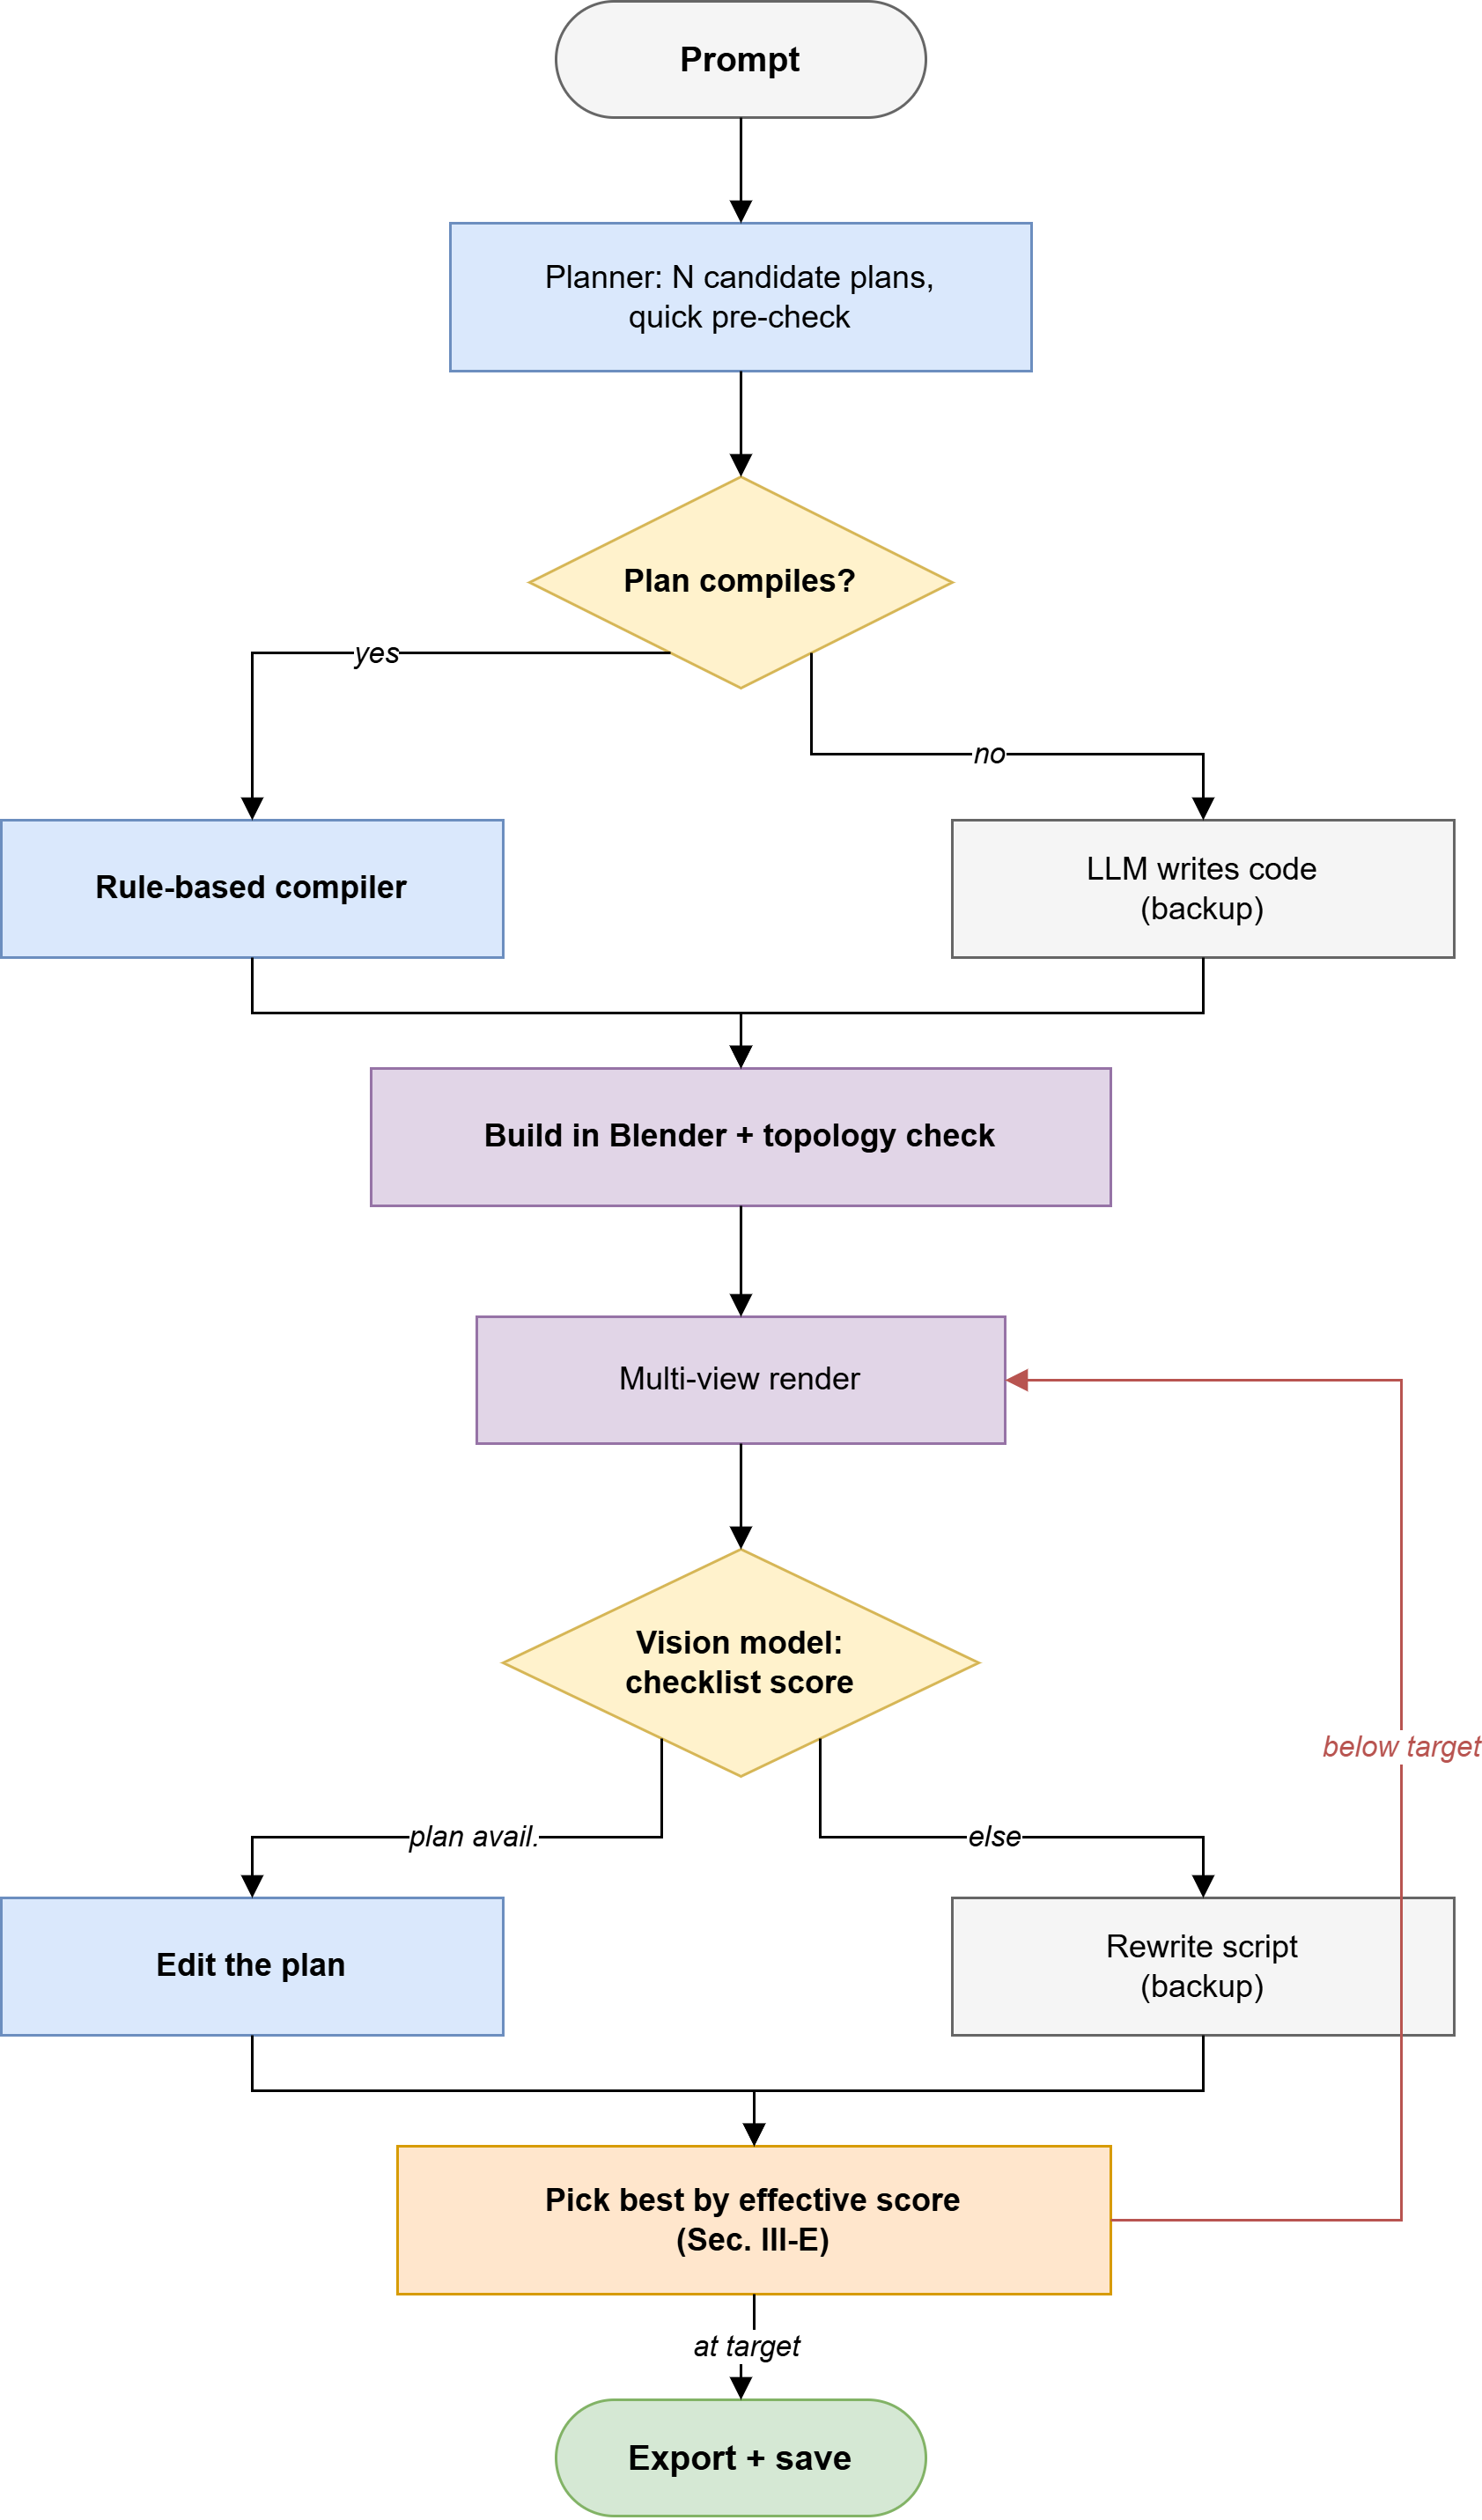
\includegraphics[width=\columnwidth]{fig1_pipeline}
\caption{The ARGUS pipeline. The compiler path (left branch) is the main path; the LLM writing code by hand (right branch) is only a backup. The repair loop after scoring also prefers editing the plan over rewriting the whole script, for the same reason.}
\label{fig:pipeline}
\end{figure}

Fig.~\ref{fig:pipeline} walks through one full run of the pipeline from start to finish. The rest of this section explains each step.

\subsection{Build Plan}
A part is a small JSON object with a name, a basic shape picked from \{\texttt{box}, \texttt{cylinder}, \texttt{sphere}, \texttt{wheel}, \texttt{bolt}, \texttt{panel}, \texttt{lathe}, \texttt{tube}, \texttt{ring}, \texttt{leaf\_card}\}, shape-specific sizes (for example, size for a box, or radius, depth, and axis for a cylinder), a position, a material name, and an \texttt{attach\_to} field pointing at its parent part. A few optional finishing fields are checked and clamped to safe ranges rather than trusted as-is: \texttt{bevel} (edge rounding, in metres), \texttt{smooth}+\texttt{crease} (smoothing with sharp edges kept where needed), and, added in this version to fix a real problem described below, \texttt{taper} and \texttt{taper\_axis}, which shrink one end of a box to make a wedge or a cone shape instead of a plain rectangular block, plus \texttt{r\_top} on cylinders for the same kind of tapering. Parts can be mirrored across an axis or repeated in a ring or a line, and the compiler expands these before building anything. Other than these placement helpers, the plan has no way to cut a hole in a shape; every part only adds material, it never subtracts it. This is a real, known limit of the system, and we say more about it in Section VI.

Before building anything in Blender, the planner writes a few candidate plans at increasing randomness, has the LLM think through the object step by step first, which is similar to how step-by-step prompting has been shown to improve LLM reasoning \cite{wei2022cot}, and scores each candidate with a quick, render-free check (a simple rule about whether parts connect and sit on the ground) so a bad layout can be thrown out before Blender is even opened.

\subsection{Rule-Based Compiler}
Every shape comes from a fixed set of functions that always build valid, clean \texttt{bmesh} geometry with UV coordinates, so there is no way for the compiler itself to create a broken edge or a bad face: the shapes are built from basic, well-tested operations (\texttt{bmesh.ops.create\_cube}, \texttt{create\_cone}, and similar), not from geometry code written fresh by an LLM that would then need to be checked separately. After placing the parts, the compiler runs a union-find check over each part's bounding box to find disconnected groups, and automatically snaps together parts that are close but not quite touching. It also adds a small, repeatable random offset to each part, based on the asset's ID and the part's ID, so building the same plan twice gives the same result, while still avoiding parts inside one object looking too identical to each other. One extra tool, called \texttt{fuse}, is the one exception to this add-only building approach: it turns a small, marked group of parts into a grid of tiny cubes and rebuilds a single smooth, sealed surface from that grid, giving a smooth, blended joint (for example, a mug handle meeting the mug body with no visible seam) where two separate parts placed side by side would leave a visible seam. This is an optional, local tool, not the system's normal way of building things; by default, ARGUS always builds an explicit polygon surface, not an implicit field or a grid of voxels.

\subsection{Materials}
The planner picks materials from a real library of photo-based textures instead of making up color values. When no photo texture matches the requested material, the compiler falls back to real, measured reflectance and roughness numbers for that kind of material, instead of a color guessed by the LLM, on the idea that a measured stand-in for the right material beats a made-up value that merely sounds right.

\subsection{Vision-Guided Repair Loop}
The finished script, whether compiled or, on the backup path, written directly by the LLM, is run inside a hidden copy of Blender. A 2$\times$2 grid of different views is rendered and scored by a vision-language model against a checklist built straight from the plan's own part list (``is the handle visible and connected to the body,'' for every listed part-to-parent connection), instead of a free-form 1--10 rating, which our own testing found to be more reliable when using a free-tier vision model. If the score is below target, the model is first asked for a short list of JSON edits to the current plan. Only when plan-editing is not possible, because the object was made by the code-writing backup, or the edit step itself fails, does the system fall back to asking for a full script rewrite. This order, plan edit first, script rewrite second, is how ARGUS keeps each fix small and easy to check, even in the backup case where it still has to touch code.

\subsection{Selection Under Uncertainty}
\label{sec:selection}
A raw score from a vision-language model is not a reliable way to choose the best result on its own, and we can show this with two real examples from our own testing instead of just claiming it. First: a compiler-built version with correctly attached, real wood photo textures scored 5/10, while a later version that lost those textures for flat, made-up color, because the fix-it prompt used to make it never mentioned materials at all, scored 6/10, and would have shipped under plain score-based picking. Second: a version that scored 8/10 under the raw score turned out, according to our own topology checker, to have a \texttt{critical} problem (floating, disconnected vertices). The vision model judges silhouette and whether parts are present; it has no way to judge whether a material looks real or whether the mesh itself is actually valid, since neither shows up as a simple yes/no answer in a checklist render.

So instead of the raw score, we pick the winner using an \emph{effective score}:
\begin{equation}
s_{\mathrm{eff}} = s_{\mathrm{vision}} - p(\sigma) + b(t)
\label{eq:effscore}
\end{equation}
where $\sigma$ is the topology problem level from our checker, with a penalty of $p(\text{clean})=0$, $p(\text{medium})=0$, $p(\text{high})=1$, $p(\text{critical})=3$, and $b(t)=\min(0.5t,\,c)$ gives credit for $t$ real textured materials, up to a limit $c$ (2 by default). In other words, how many score points a real photo texture is ``worth'' is a choice we made and can tune, not a fixed fact. A new candidate only replaces the current best if its effective score is strictly higher; if it does not clear that bar, it is turned down and the exact reason (a topology problem, or fewer textures than before) is written to the run log instead of just quietly dropped. Checked against both real examples above, this one rule stops an already-textured, clean object from losing to a small raw-score bump, and stops a broken object from winning just because its silhouette looked fine.

\subsection{Fallback Chain and Resilience}
When the compiler path is not available, script writing tries a list of backup AI providers one after another, a first try that can see images, then several text-only backups, and rotates through up to ten API keys per provider to work around rate limits. A set of hand-written backup scripts, chosen by matching keywords in the request, is used as a last resort for object types the planner cannot otherwise handle; these used to be a real source of the texture-losing bug described in Section III-E. A small, careful add-on step now matches already-downloaded photo materials onto these backup scripts' flat, made-up materials by comparing the words in their names, and it never touches a material the script already textured correctly.

\subsection{Interactive Control}
A single run can take tens of minutes. Letting the user cancel a run uses the same shared checkpoint the pipeline's own time-limit check already uses, so cancelling takes effect at the next natural break in the loop, and the pipeline still finishes exporting and checking whatever was already built, instead of just killing the process outright.

\section{Implementation}
The main program is a Python process that drives a hidden copy of Blender 5.0 through a subprocess, and exports GLB, FBX, and a native \texttt{.blend} file. The desktop app is built with Tauri and React, talking to a FastAPI backend that sends pipeline progress as a stream of typed events, stage changes, key/value updates, scores, and the final result, replacing an older setup where two separate parts of the app each tried to read the same plain-text console output with their own pattern-matching code, a fragile setup this version removes completely instead of patching around. The test suite (Section V) runs each (prompt, setting) pair as its own separate process, since the output folder is set once when the Python module first loads, so testing each pair on its own needs a brand-new process; the numbers are then computed directly from the exported glTF file's own data (triangle count, vertex count, material count, embedded image count) instead of by rendering again, so re-checking a finished set of results costs nothing and can never disagree with itself between runs.

\section{Evaluation}
\label{sec:eval}

\subsection{Test Set}
We built a 30-prompt test set split into three difficulty levels based on how complex the shape actually is, not how hard it sounds: \emph{simple} (one main shape, like a traffic cone), \emph{moderate} (several parts put together, several of which have a matching, hand-checked reference in the system's own shape library, like a park bench), and \emph{complex} (jointed, irregular, or organic-looking shapes with no matching reference, like a desk lamp or a steam train). This paper reports a first, smaller test run of 5 prompts per level (15 total) using the system's normal settings. The full 30-prompt set and the rest of the comparison settings are listed as the next step in Section VI.

\subsection{Metrics}
All shape and material numbers come straight from the exported glTF file: triangle count, vertex count, mesh count, material count, textured-material count (materials that use a real image), and embedded image count. The topology problem level (clean/medium/high/critical) and whether the object sits properly on the ground both come from the checker's report made while Blender was building the object. Visual quality is the vision-language checklist score explained in Section III. We also report how often the taper and \texttt{r\_top} shape options actually get used, as a check on whether just adding an option to the plan format is enough to make the planner use it: before this update, 0 of 248 boxes in a snapshot of earlier results used any taper at all, since the field did not exist yet, and only 4 of 98 cylinders (4.1\%) used the older \texttt{r\_top} field even though it was already available. So just adding a feature to the format clearly is not enough on its own to get the planner to actually use it.

\subsection{Results}
Table~\ref{tab:overall} sums up the 15-prompt test run; Table~\ref{tab:perasset} lists every single result. All 15 prompts produced a real, exportable object (100\% build completion). No object scored \texttt{critical} on topology. 87\% of objects came out with clean topology, and 87\% had at least one real textured material. Against the new, higher target score of 8/10, using the effective score from Section III-E, 9 of 15 (60\%) hit or beat that target. On the raw vision score alone only 5 of 15 (33\%) reach 8/10; the difference is entirely the effective score's texture bonus, which is what lifts a clean, well-textured build over the bar and is precisely the correction Section III-E argues for. Against the system's older default target of 7 on the raw score, 9 of 15 (60\%) also qualified. Both figures are computed by \texttt{eval/metrics.py:effective\_score()}, which mirrors the pipeline's own Eq.~1, and are reproducible with \texttt{python -m eval.report}; an earlier draft of this paper quoted the raw 33\% while labelling it the effective score, because the figure was derived by hand from Table~\ref{tab:perasset} rather than computed from the logged results.

\begin{table}[t]
\centering
\caption{Pilot test run summary (15 prompts, normal settings)}
\label{tab:overall}
\begin{tabular}{lccc}
\toprule
Metric & Simple & Moderate & Complex \\
\midrule
$n$ & 5 & 5 & 5 \\
Build completion & 100\% & 100\% & 100\% \\
Mean visual score & 6.4 & \textbf{7.6} & 6.0 \\
$\geq$7/10 & 60\% & 80\% & 40\% \\
Clean topology & 80\% & \textbf{100\%} & 80\% \\
Critical topology & 0\% & 0\% & 0\% \\
Textured & \textbf{100\%} & 60\% & \textbf{100\%} \\
Mean triangles & 3{,}565 & 20{,}157 & 63{,}856 \\
Mean time (s) & 599 & 736 & 1{,}027 \\
\bottomrule
\end{tabular}
\end{table}

\begin{table*}[t]
\centering
\caption{Result for every asset in the pilot test run}
\label{tab:perasset}
\small
\begin{tabular}{lllccccc}
\toprule
ID & Level & Prompt & Score & Topology & Textures & Triangles & Time (s) \\
\midrule
b01 & simple   & a wooden crate                 & 7 & high  & 5  & 7{,}600   & 669 \\
b02 & simple   & a steel oil drum               & 7 & clean & 1  & 5{,}624   & 897 \\
b03 & simple   & a traffic cone                 & 5 & clean & 4  & 1{,}276   & 413 \\
b04 & simple   & a cardboard shipping box       & 6 & clean & 9  & 1{,}820   & 678 \\
b05 & simple   & a concrete cinder block        & 7 & clean & 1  & 1{,}504   & 335 \\
b09 & moderate & a cast iron fire hydrant       & 8 & clean & 0  & 18{,}672  & 242 \\
b10 & moderate & a rustic park bench            & 5 & clean & 3  & 5{,}952   & 1{,}334 \\
b11 & moderate & a fire extinguisher            & 8 & clean & 0  & 6{,}748   & 1{,}422 \\
b12 & moderate & a street lamp post             & 8 & clean & 17 & 4{,}216   & 387 \\
b13 & moderate & a wooden step stool            & \textbf{9} & clean & 1  & 65{,}196  & 294 \\
b21 & complex  & a steam locomotive engine      & 6 & high  & 25 & 21{,}096  & 766 \\
b22 & complex  & a wooden windmill              & 8 & clean & 5  & 4{,}996   & 776 \\
b23 & complex  & an anglepoise desk lamp        & 7 & clean & 14 & 3{,}560   & 1{,}641 \\
b24 & complex  & a vintage gas pump             & \textbf{3} & clean & 19 & \textbf{281{,}182} & 938 \\
b25 & complex  & a wheelbarrow                  & 6 & clean & 14 & 8{,}444   & 1{,}016 \\
\bottomrule
\end{tabular}
\end{table*}

\begin{figure}[t]
\centering
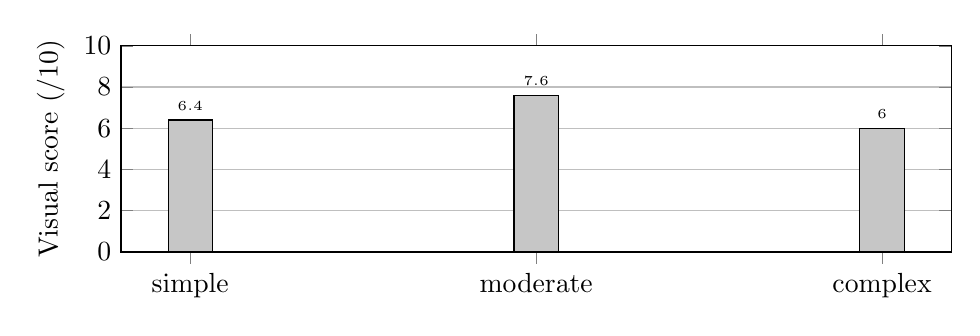
\begin{tikzpicture}
\begin{axis}[
  ybar, width=\columnwidth, height=4.2cm,
  ylabel={Visual score (/10)}, ymin=0, ymax=10,
  symbolic x coords={simple,moderate,complex},
  xtick=data, nodes near coords, nodes near coords style={font=\tiny},
  bar width=16pt, ymajorgrids, axis on top=false,
]
\addplot[fill=gray!45] coordinates {(simple,6.4) (moderate,7.6) (complex,6.0)};
\end{axis}
\end{tikzpicture}
\caption{Average visual score by difficulty level. The moderate level beats the simple level even though it is harder by definition, discussed in Section~\ref{sec:qualitative}.}
\label{fig:tierbar}
\end{figure}

\subsection{Qualitative Analysis}
\label{sec:qualitative}
Two results in Table~\ref{tab:perasset} are worth a closer look.

\emph{Moderate beats simple.} Fig.~\ref{fig:tierbar} shows the moderate difficulty level scoring higher on average (7.6) than the simple level (6.4), even though moderate prompts are, by definition, harder to build. Four of the five moderate prompts have a hand-checked reference in the shape library. We think the gap comes from those reference shapes mattering more to the final quality than raw shape simplicity does, which tells us something about where the system's real strength currently comes from, and it is not what the difficulty grouping predicted.

\emph{The gas-pump outlier.} b24 scored 3/10, the lowest score in the whole test run, even though it had clean topology and 19 real textured materials, at 281{,}182 triangles: about $4.3\times$ more than the next-highest object in the entire run (b13, at 65{,}196). A low score next to clean topology and full texturing does not match the usual failure pattern this paper focuses on in Section III-E, a high score hiding a real problem. We think this is instead a separate, unrelated geometry bug, most likely a modifier stack that ran out of control, or an unlimited part-repeating step tied to how many parts this specific prompt asked for. Our current numbers can flag this case, since the triangle count is an obvious outlier, but cannot explain it. We are reporting it honestly instead of leaving it out.

Fig.~\ref{fig:qualgrid} turns the topology numbers in Table~\ref{tab:overall} into something you can actually look at, showing six objects from the test run in both their finished, rendered form and as raw wireframe geometry.

\begin{figure*}[t]
\centering
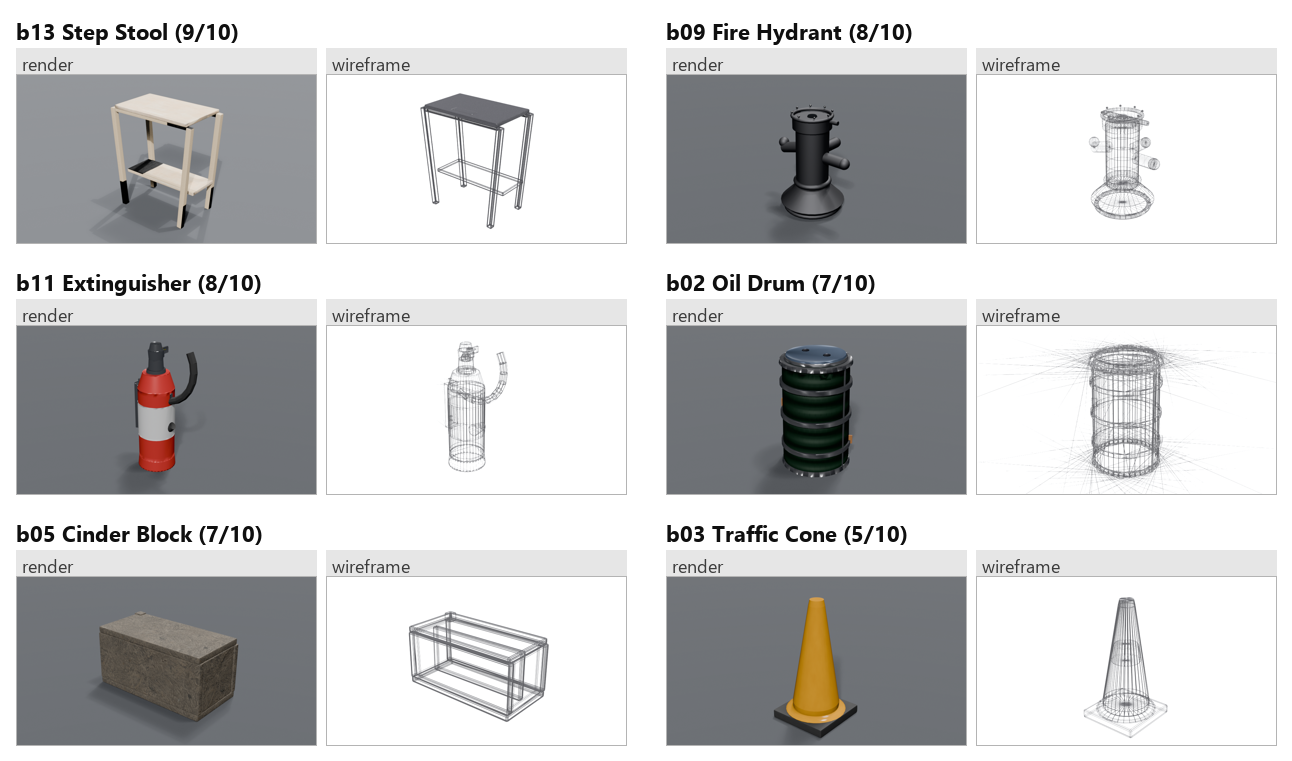
\includegraphics[width=0.92\textwidth]{fig3_qualitative_grid}
\caption{Render and wireframe pairs, from the same camera angle, for six objects from the test run: the highest-scoring result at each difficulty level plus three more objects with clean topology. The wireframes are real renders of each object's exported geometry, not drawings made to illustrate the idea.}
\label{fig:qualgrid}
\end{figure*}

\subsection{An Infrastructure Finding}
\label{sec:dns}
While collecting results with nobody watching, 12 of the 30 raw attempts behind our 15 reported cells failed with a DNS lookup error. Every one recovered on retry, so all 15 cells are backed by a clean run, but the cause is worth reporting because we initially misdiagnosed it. Our first explanation was self-inflicted congestion: the fallback chain fires roughly fifteen hostname lookups in quick succession whenever it walks several providers in a row, and we assumed that burst was overwhelming the local resolver. It was not. One of the configured providers, GitHub Models, had been permanently retired upstream --- its endpoint (\texttt{models.inference.ai.azure.com}) was deprecated in July 2025 and the service was shut down entirely in July 2026 --- so the hostname no longer exists at all. A direct lookup returns NXDOMAIN, with no concurrency and no load. Every generation was paying a full connection-failure cycle on a dead provider before falling through to a live one.

The lesson is not the dead endpoint itself but what it did to our measurements. Our environment-failure detector flagged a cell whenever a known network-failure signature appeared \emph{anywhere} in its log. That was sound while such failures were genuinely transient, but a permanently dead provider puts the signature in every log, including logs of runs that fell through to a working provider and completed perfectly. The detector therefore began excluding good results as environment failures --- 149 of them in one sweep --- which would have silently emptied the very quality numbers it was built to protect. The fix is to require corroboration: a run counts as an environment failure only if the signature appears \emph{and} the run failed to produce a scored asset. We report this because the failure mode generalises past our own bug. A resilience mechanism that survives a dead dependency by design will keep succeeding quietly, and its logs will keep carrying that dependency's error text forever; any detector keyed on log text alone will drift from measuring the environment to measuring the fallback chain's own noise floor.

\section{Threats to Validity and Limitations}
\label{sec:limits}
We are putting these limits up front instead of burying them at the end, because several of them change how the results above should be read.

\begin{itemize}
\item \textbf{No comparison tests have been run yet.} The test suite already supports nine on/off settings (compiler vs.\ LLM code-writing as the main path, with/without the visual repair loop, with/without the outer full-rebuild loop, how many candidate plans to try, two-step planning, the checklist-based judge, the reference image, and edge rounding) as simple settings that need no code changes to turn on or off; but none of them have actually been run against the full test set for this paper. We cannot yet say which specific part of the system is responsible for the quality we are reporting.
\item \textbf{No comparison against other systems yet.} The code already has a place to plug in feed-forward neural systems (TripoSR, TRELLIS, Hunyuan3D 2.0) for comparison, and the design lines up well against LLM-code systems (LL3M, SceneCraft), but we have not run a head-to-head test against either group yet.
\item \textbf{One judge, no human study.} The only quality judge is a free-tier vision-language model. We do not yet have data on how consistent or repeatable that judge is; earlier testing saw the exact same rendered object get a different score from what should have been the same kind of scoring call within a single run, which is exactly why Section III-E's picking rule does not trust the raw score alone. But the judge's overall accuracy still has not been checked against real human opinions.
\item \textbf{Small sample size.} 15 results is not enough to prove anything statistically; every pattern we noticed in Section V-D is something worth testing further, not a proven finding yet.
\item \textbf{Limited scope.} The test set and the plan format are built for still, hard-surface, mostly non-living objects. Living or organic shapes, characters, and full scenes with multiple objects are simply out of scope by design, not something we tried and failed at.
\item \textbf{No cutting holes.} The plan format can only add material, aside from the one optional fuse tool; holes, notches, and slots, which are common on real hard-surface objects, cannot be described yet.
\item \textbf{Results may not repeat exactly elsewhere.} All tests used free-tier API limits on one single computer; the exact timings and the network-failure pattern we found (Section V-E) might not show up the same way on paid plans or with different AI providers.
\end{itemize}

\section{Future Work}
The next real step is running the comparison tests the test suite already supports, across the full 30-prompt set, followed by a direct comparison against TripoSR, TRELLIS, Hunyuan3D 2.0, and an LLM-code system, all on the same prompts using the same numbers, plus a small study with real human raters to check how accurate the vision-language judge actually is. On the shape side, we want to add a real hole-cutting tool to the plan format, and look into a signed-distance-field method for a wider range of part joints than the one optional fuse tool currently supports, without replacing the plain polygon-based approach as the default for hard-surface parts, where it is still the better fit.

\section{Conclusion}
ARGUS splits apart two jobs that earlier LLM-scripted 3D systems mixed into one: spatial planning and code-writing. It turns spatial planning into a plan an LLM writes and a compiler builds, and shows, using real, measured examples instead of just claims, that a raw vision-language quality score by itself is not a safe way to pick a winner and needs to be corrected using real topology and material information. This is a systems paper reporting a first test run: the architecture and the picking rule are both built, tested, and measured on a real 15-prompt run with 100\% build completion and zero critical-topology results. The comparison tests and baseline comparisons that would show exactly which part of the system deserves credit for that result are listed plainly as the next step, not finished yet.

\section*{Acknowledgment}
The author thanks Mr.\ Anmol Pandey, Assistant Professor, Department of Computer Engineering, Sikkim Institute of Science and Technology, for guiding the earlier version of this system \cite{dahal2026thesis} that this paper builds on.

\bibliographystyle{IEEEtran}
\bibliography{references}

\end{document}
